\documentclass[a4paper,titlepage,12pt]{article}
\usepackage[utf8]{inputenc}
\usepackage{todonotes}
\usepackage{url}
\usepackage{listings}
\usepackage{color}
\usepackage{subcaption}
\usepackage[linesnumbered,ruled,vlined]{algorithm2e}
\begin{document}
 
\newcommand{\horrule}[1]{\rule{\linewidth}{#1}}     % Horizontal rule

\title{
        %\vspace{-1in}  
        \usefont{OT1}{bch}{b}{n}
        \normalfont \normalsize \textsc{KU Leuven} \\ [25pt]
        \normalfont \normalsize \textsc{Computer Vision} 
        \horrule{2pt} \\[0.5cm]
        \huge Final Project: Incisor Segmentation \\
        \horrule{2pt} \\[0.5cm]
}
\author{
        \normalfont            
        Joran Van de Woestijne (r0378602)\\
        Tim Van Den Broecke (r0296620)
}
\date{August 2017}
 
\maketitle

\newpage
\tableofcontents
\thispagestyle{empty}
\newpage
\setcounter{page}{1}

\section{Introduction}

This report discusses our solution for the Incisor Segmentation project for the Computer Vision course.
The goal of this project was to develop a model based segmentation approach, capable of segmenting the upper and lower incisors in panoramic radiographs.
We achieved this by utilizing the Active Shape Models approach, as it was first presented by Cootes et al \cite{cootes2000introduction}.
This report is structured as follows: 
Section \ref{sec:shape} starts of by discussing the deformable shape model, which is followed up by Section \ref{sec:preproc} concerning the pre-processing of the dental radiographs. Section \ref{sec:fitting} presents the actual model fitting algorithm, with the evaluation of the fitting presented in Section \ref{sec:eval}.

\section{Shape Model}
\label{sec:shape}
We use two models in our algorithm. One describes the mean and variation of all four upper teeth (incisors 1-4), the other describes the lower teeth (incisors 5-8). 

The choice for two models containing four incisors each, as opposed to one model per tooth, comes from two main reasons that both stem from simple empirical observations about the human dental structure. The first is that the upper and lower incisors are always found next to eachother and in the same order. Natural variations on the spacing between them, their height differences and sizes are all captured in our final model description. Our approach ensures that teeth will never be marked out of order within the model, even when some overlap. The second observation is that natural variations don't favor one side over the other and thus we expect a symmetric model. Including mirrored examples during training is one way to incorporate this information. Our model adds to the effect by also enforcing symmetry in the variation in spacing, height and size.

The model construction happens in two steps, as described by Cootes in \cite{cootes2000introduction} (ignoring the labelling as it has been performed for us). First, we align all the shapes. This means making all example sets of four incisors (either all upper or all lower) neutral with regards to translation, rotation and scale. Afterwards, we perform a principal component analysis (PCA) on the aligned shapes to acquire a robust description of the average upper/lower incisors and the way they vary in shape. 

\subsection{Shape alignment}
Starting from the labelled set of images and their eight manually landmarked incisors, we group the upper and lower landmarks and combine them into one shape vector. This vector contains the coordinates of 160 ($= 4\times 40$ points per landmark) points. When testing the performance of our algorithm for a specific image, we remove it and its mirrored version from the training set. We are then left with 26 training examples per model (upper or lower) for an image.

We take the first example as the initial mean shape estimate and normalize it. Using Procrustes analysis, we refine the estimate using the other examples until it converges. At the start of each refinement step we align all examples with the new mean so that when the procedure has converged, we have acquired a fully aligned set of examples. We see the process illustrated in Figure \ref{fig:align} when training for image 4. Notice that the slight tilt of the first example (and therefore also the initial mean estimate) has cascaded into the full alignment set. This can not be prevented using our technique.

\begin{figure}
	\centering
	\begin{subfigure}{\linewidth}
		\centering
		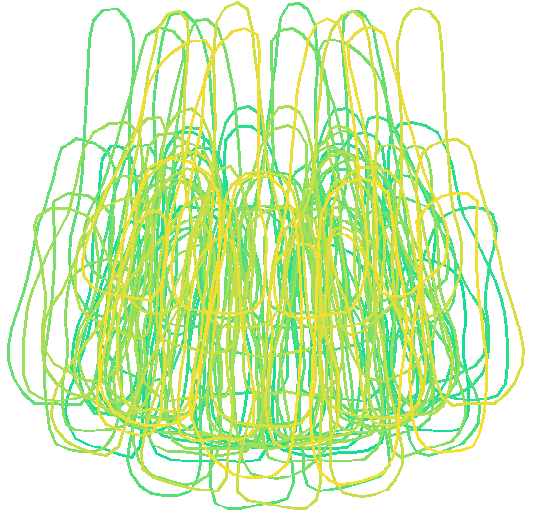
\includegraphics[width=0.4\linewidth]{shape/upper_init}
		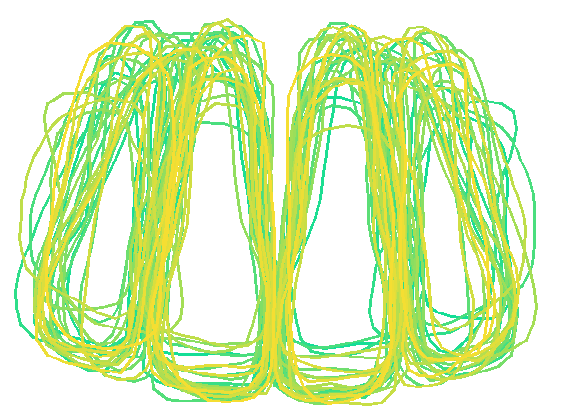
\includegraphics[width=0.4\linewidth]{shape/upper_aligned}
		\caption{Model 1: upper incisors}
	\end{subfigure}
	\begin{subfigure}{\linewidth}
		\centering
		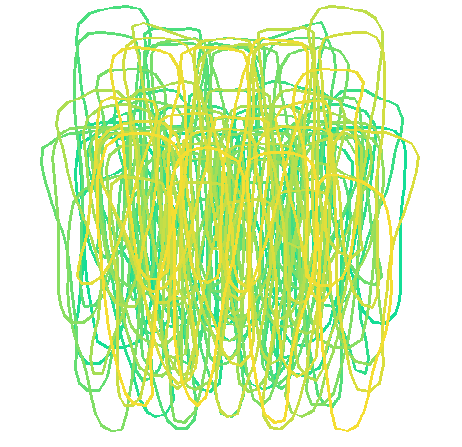
\includegraphics[width=0.4\linewidth]{shape/lower_init}
		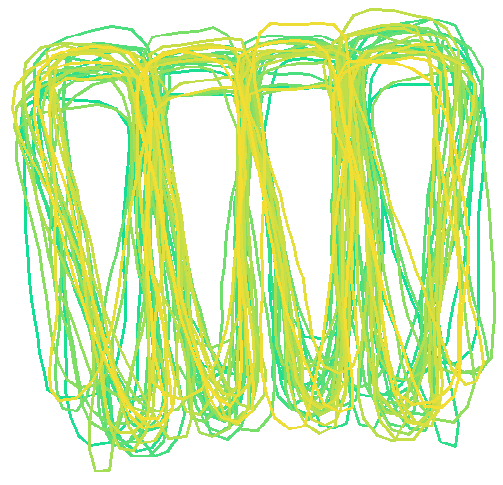
\includegraphics[width=0.4\linewidth]{shape/lower_aligned}
		\caption{Model 2: lower incisors}
	\end{subfigure}
	\caption{Our two models before and after alignment. Examples 4 and 18 (mirrored 4) were left out. On the left we see the original landmarks simply superposed in one image, each with their own color gradient. On the right, we see the the aligned models with their same respective color. }
	\label{fig:align}
\end{figure}

\subsection{PCA}
After aligning our training set, we want to extract statistical properties from it describing the mean shape of a model and the typical variation found within them. A principal component analysis delivers just that. We create a procedure that takes a training set of models and produces a PCA model of the set and a description of the training set in terms of said model (called the \emph{reduced training set}). The model is used throughout the algorithm to correct new estimated fits. The terms in the reduced training set are analysed to determine a plausible range for models. We confirm in Figure \ref{fig:stdvar} that (positive or negative) three times the standard deviation on each term captures the range of plausible shapes. 

To determine the number of modes we need for the PCA, we provide a dynamic procedure. It first calculates all eigenvalues in descending order and then searches for the number of values needed to cover 95\% of the shape variation inside the training set. We plot the coverage per number of modes used to train for image 4 in Figure \ref{fig:coverage}. 

\begin{figure}
	\centering
	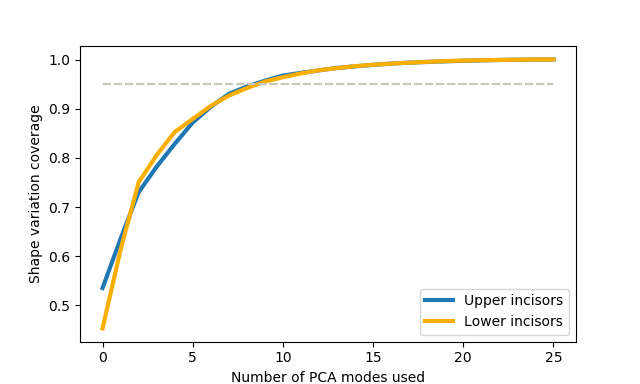
\includegraphics[width=0.75\linewidth]{shape/coverage5}
	\caption{Coverage plot for our two models. We see that we need 10 modes of our PCA in order to cover 95\% of shape variations in the training set. }
	\label{fig:coverage}
\end{figure}

\begin{figure}
	\centering
	\begin{subfigure}{\linewidth}
		\centering
		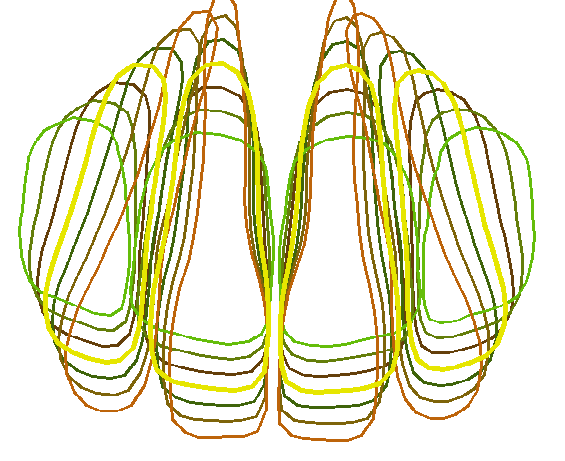
\includegraphics[width=0.19\linewidth]{shape/up_pca1}
		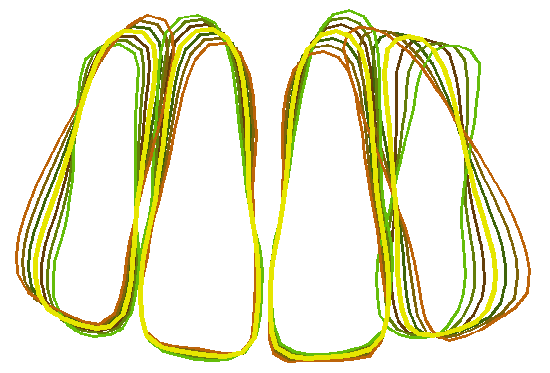
\includegraphics[width=0.19\linewidth]{shape/up_pca2}
		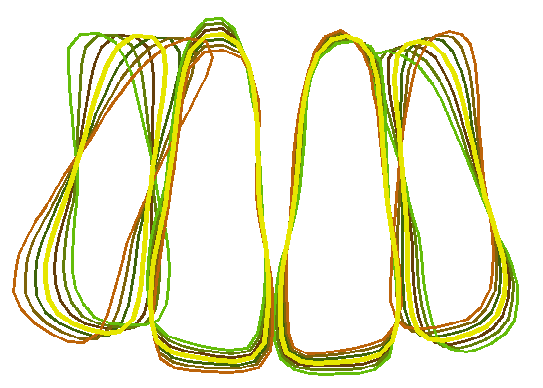
\includegraphics[width=0.19\linewidth]{shape/up_pca3}
		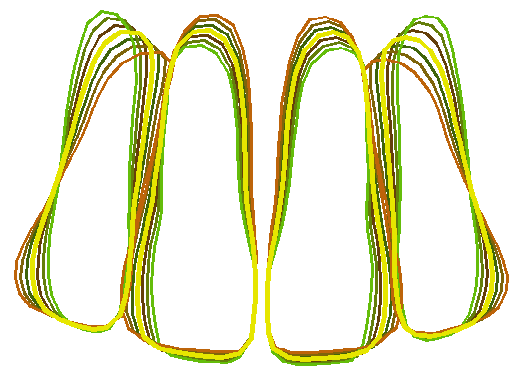
\includegraphics[width=0.19\linewidth]{shape/up_pca4}
		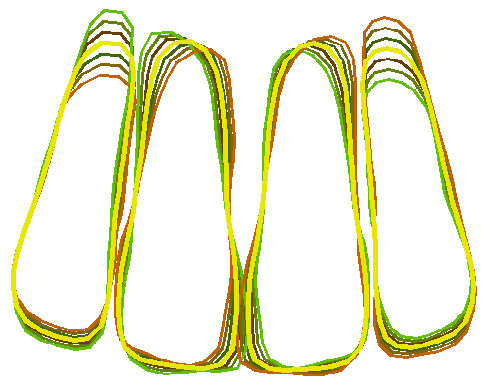
\includegraphics[width=0.19\linewidth]{shape/up_pca5}
		\caption{Model 1: upper incisors}
	\end{subfigure}
	\begin{subfigure}{\linewidth}
		\centering
		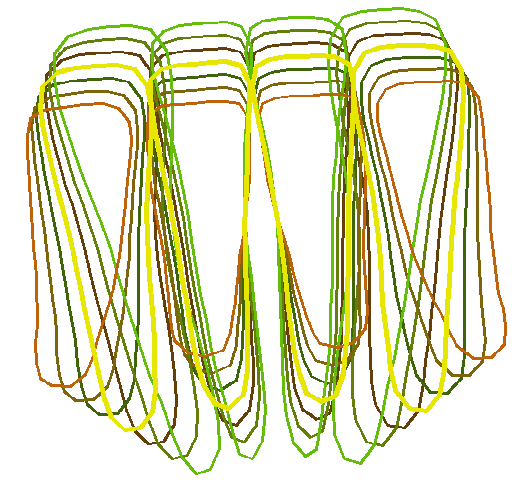
\includegraphics[width=0.19\linewidth]{shape/low_pca1}
		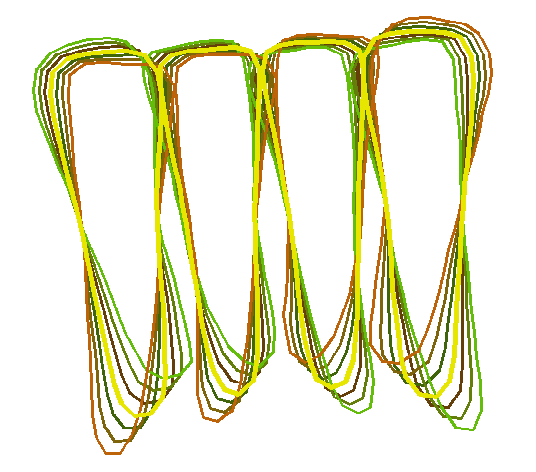
\includegraphics[width=0.19\linewidth]{shape/low_pca2}
		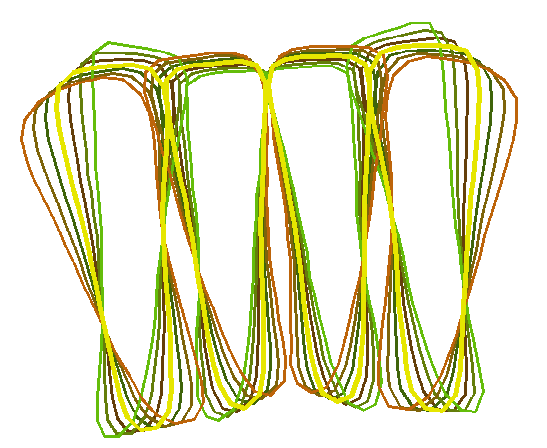
\includegraphics[width=0.19\linewidth]{shape/low_pca3}
		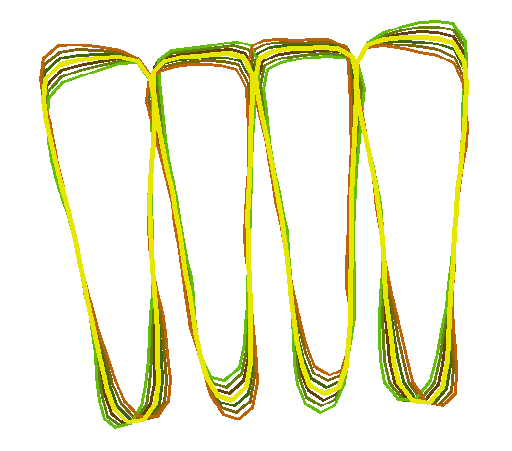
\includegraphics[width=0.19\linewidth]{shape/low_pca4}
		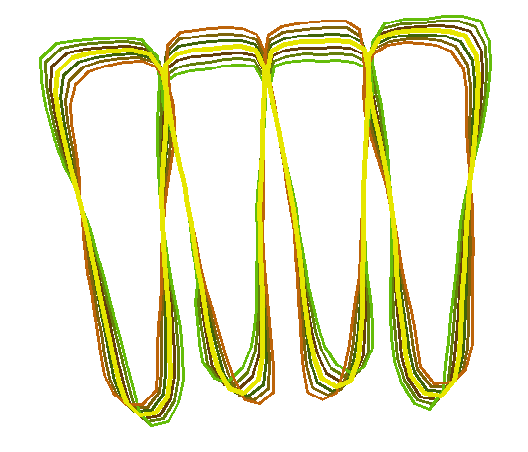
\includegraphics[width=0.19\linewidth]{shape/low_pca5}
		\caption{Model 2: lower incisors}
	\end{subfigure}
	\caption{The five main principal components in order of our two models, excluding examples 4 and 18. The mean shape is shown in yellow. Each component is shown with a scaling between -3 and +3 times the standard deviation of the component. }
	\label{fig:stdvar}
\end{figure}

\section{Radiograph pre-processing}
\label{sec:preproc}

Dental radiographs are inherently noisy and contain too much information when just focusing on locating the upper and lower incisors.
For instance, all the teeth (not just the incisors), the jaw and the nose are present in the radiographs.
To reduce these radiographs to a more suitable size for our application, we crop them based on domain knowledge so that only the smaller region around the four incisors remains.

After the size reduction, the radiographs still need to be de-noised so that it's easier for our algorithm to detect the edges.
We achieve this by using the technique proposed in \textit{Noise Removal and Contrast Enhancement for X-Ray Images} by Huang et al \cite{JBEMI1893}.
The algorithm proposed by Huang et al is visualised in Figure \ref{preprocessalgo}. This technique first starts off by applying an adaptive median filter to reduce the impulsive (salt-and-pepper) noise, after which a bilateral filter is used to suppress the Gaussian noise while also preserving the edges of the image.
After the noise suppression step, the radiograph is sharpened by a mathematical morphology, here a top hat and bottom hat transform.
The top hat transform enhances the brighter regions of the radiograph, whereas the bottom hat enhances the darker regions.
Finally, the contrast of the radiograph is enhanced by applying a contrast limited adaptive histogram equalization (CLAHE).
To detect the edges of the dental radiograph, a Sobel operator is used, detecting the gradients in the x and y direction.
The results of applying the different pre-processing steps on a dental radiograph can be observed in Figure \ref{preprocess}. 


\begin{figure}
\centering
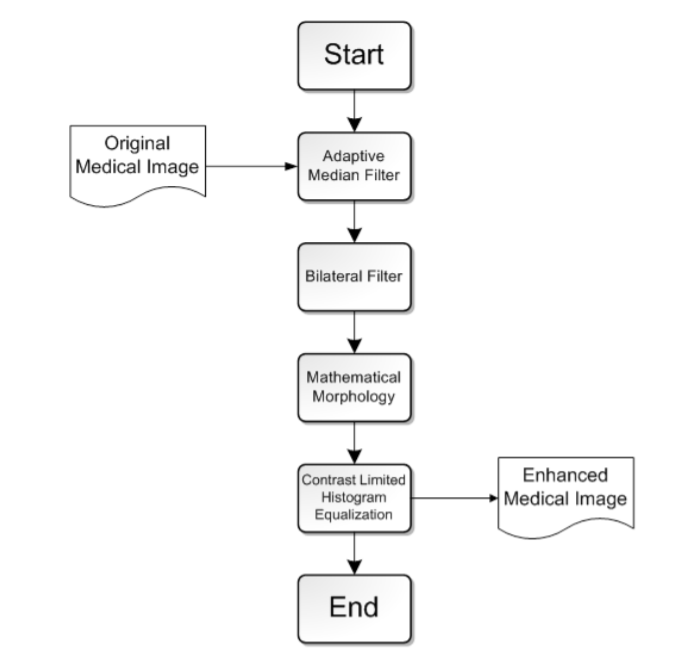
\includegraphics[width=0.7\linewidth]{preprocess/algorithm.png}
  \caption{
		The algorithm proposed by Huang et al \cite{JBEMI1893} for denoising dental radiographs. The algorithm has four steps, with a top hat transform and a bottom hat transform representing the mathematical morphology step. } \label{preprocessalgo}
\end{figure}

\begin{figure}
  \centering
	\begin{minipage}[b]{0.23\linewidth}
		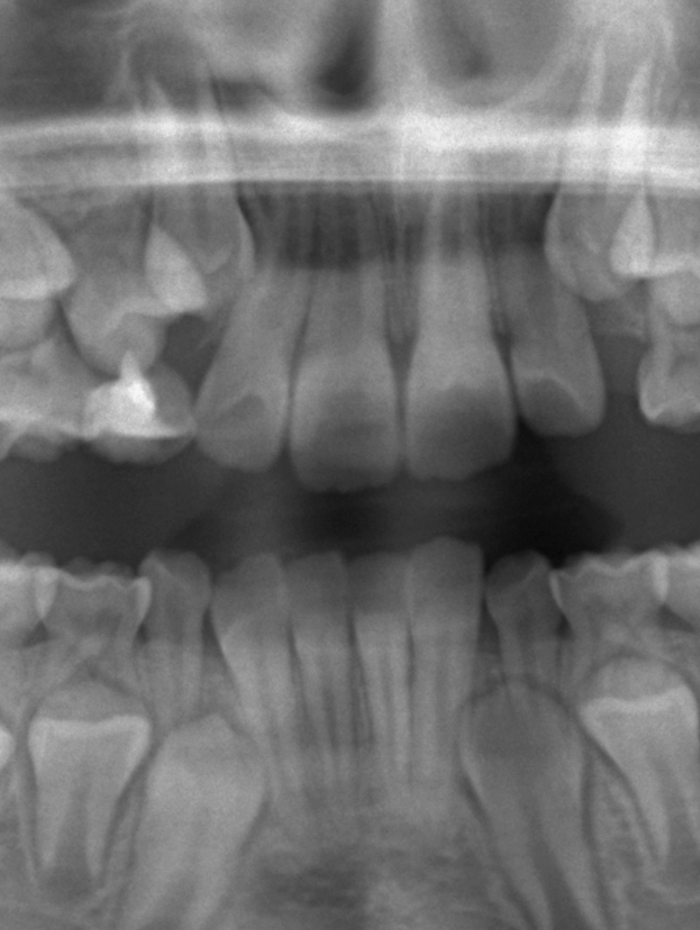
\includegraphics[width=\linewidth]{preprocess/original.png}
		\subcaption{Cropped}
	\end{minipage}
	\begin{minipage}[b]{0.23\linewidth}
		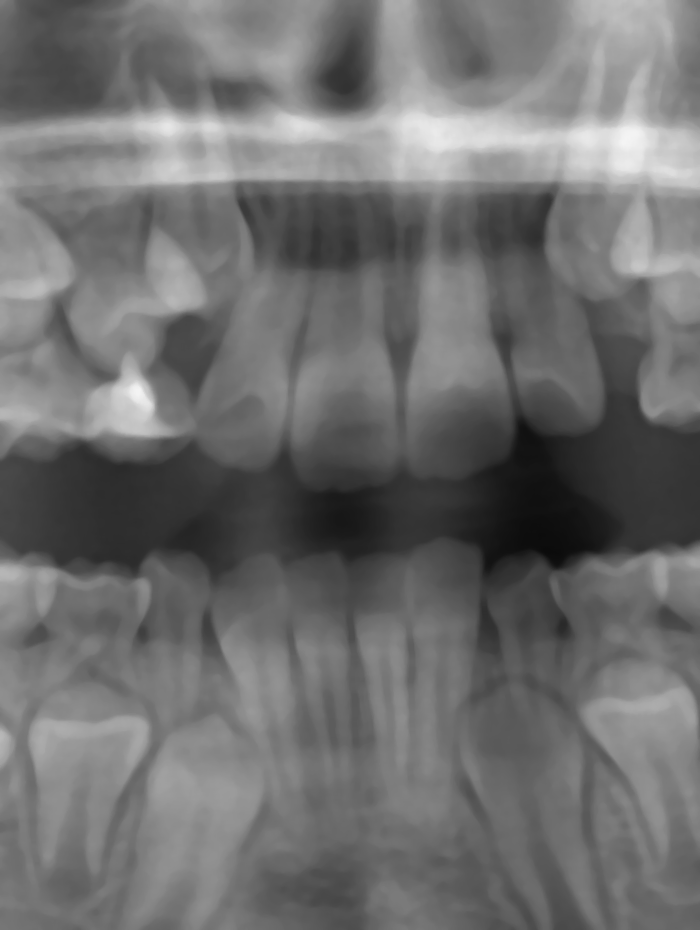
\includegraphics[width=\linewidth]{preprocess/median.png}
		\subcaption{Median filter}
	\end{minipage}
	\begin{minipage}[b]{0.23\linewidth}
		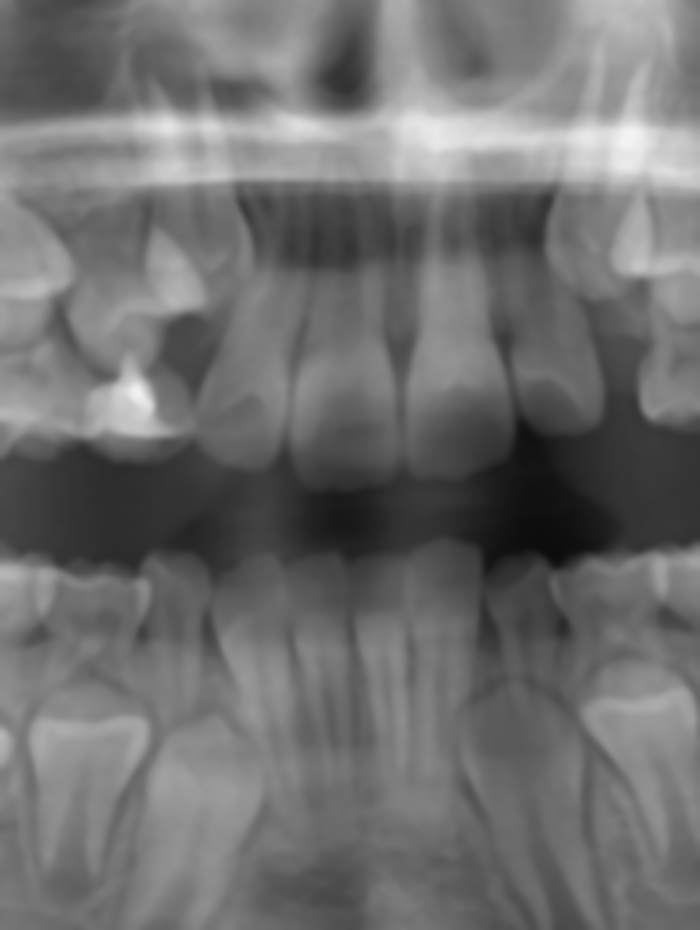
\includegraphics[width=\linewidth]{preprocess/bilateral.png}
		\subcaption{Bilateral Filter}
	\end{minipage}
	\begin{minipage}[b]{0.23\linewidth}
		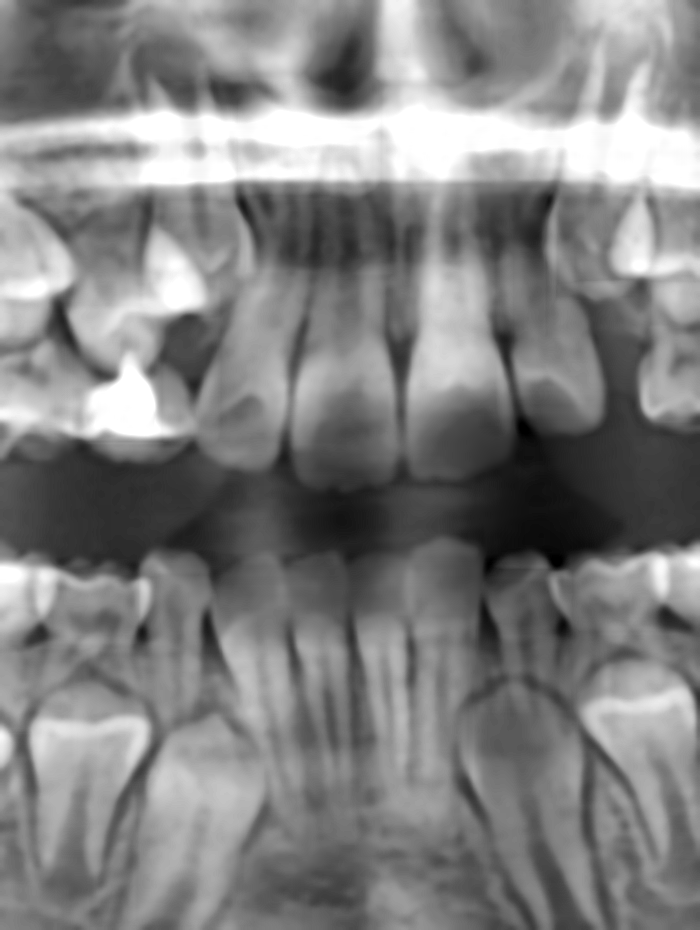
\includegraphics[width=\linewidth]{preprocess/hats.png}
		\subcaption{Morphology}
	\end{minipage}
	\begin{minipage}[b]{0.23\linewidth}
		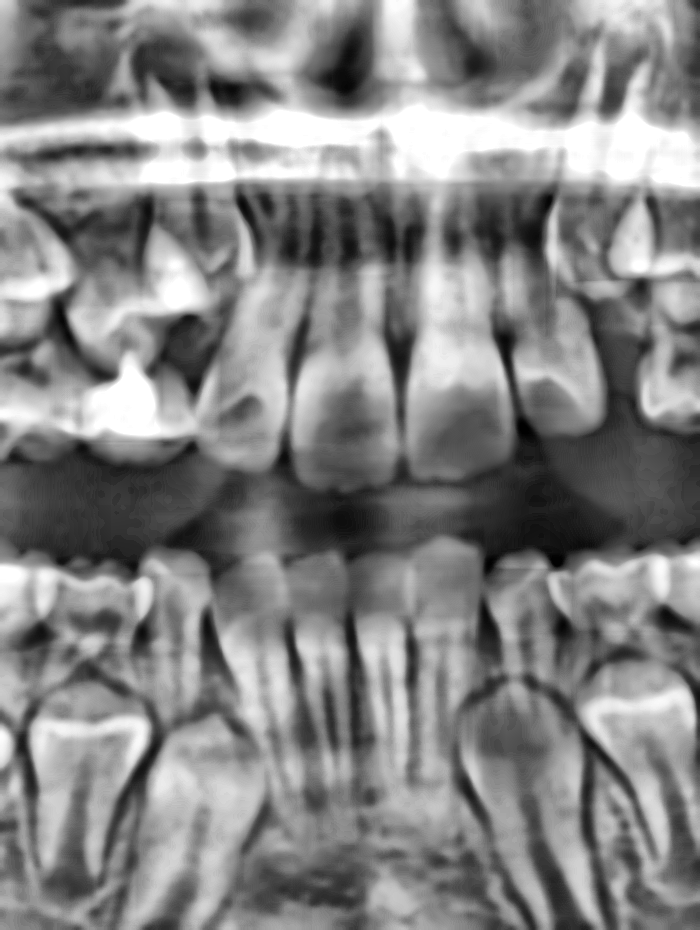
\includegraphics[width=\linewidth]{preprocess/clahe.png}
		\subcaption{CLAHE}
	\end{minipage}
	\begin{minipage}[b]{0.23\linewidth}
		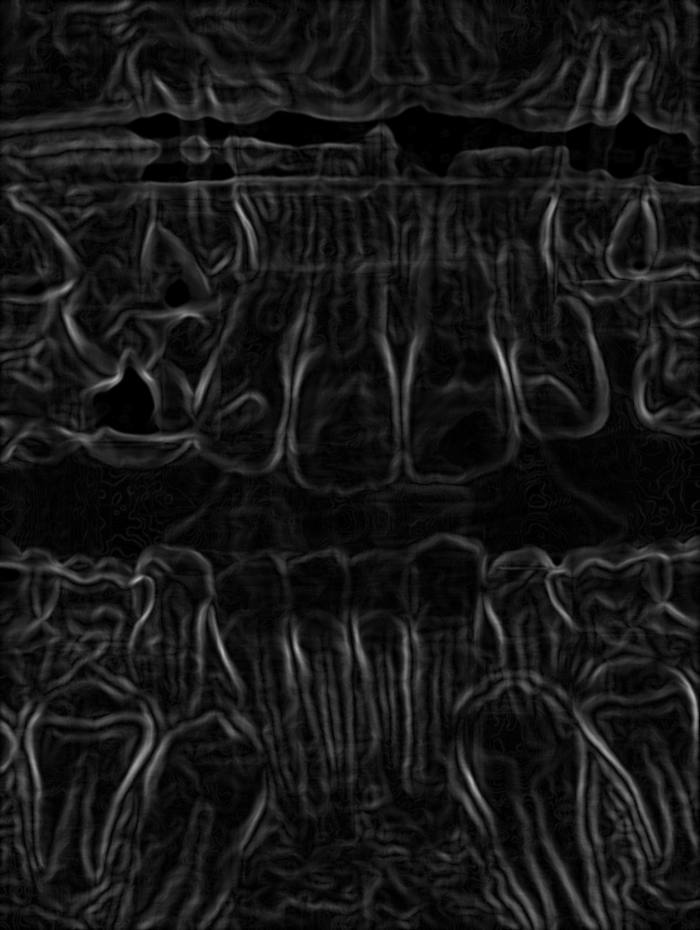
\includegraphics[width=\linewidth]{preprocess/gradients.png}
		\subcaption{Edges (Sobel)}
	\end{minipage}
  \caption{
		The results of the different pre-processing steps visualised when applied on dental radiograph 3.
		(a) shows the original image after cropping, (b) shows (a) after applying the adaptive median filter, (c) adds the bilateral filter onto the result of (b), (d) performs the mathematical morphology (top hat and bottom hat) on (c), and (e) finally applies CLAHE. A Sobel operator is used to detect the edges, which is visualised in (f).} \label{preprocess}
\end{figure}


\section{Fitting model to image}
\label{sec:fitting}
To fit our model to an image, we have to find the model instance $x =T_{(X_t,Y_t,s,\theta)}(\bar{x} + Pb)$ that most accurately aligns with the incisors in the image.
This translates to finding the pose parameters $T_{(X_t,Y_t,s,\theta)}$ and the shape parameters $b$.
This is achieved in two steps: In the first step, an initial estimate for the pose parameters is obtained, which is discussed in Section \ref{subsec:initial} . The second step finally fits the model to the image by applying the Active Shape Model algorithm, which is discussed in Section \ref{subsec:ASM}

\subsection{Initial pose estimate}
\label{subsec:initial}

To determine an initial estimate for the pose parameters $T_{(X_t,Y_t,s,\theta)}$, we need to find an estimate for the horizontal offset $X_t$, the vertical offset $Y_t$, the scale $s$ and the rotation $\theta$.

\paragraph{Scale and rotation}

To find an initial estimate for the scale and rotation, we use domain knowledge. A good scale was empirically determined, and the rotation is chosen so that the teeth are positioned vertically.

\paragraph{Vertical offset}

To find the vertical offset $Y_t$, we utilise the jaw separation of the radiograph.
This is accomplished by first finding the jaw separation that separates the upper incisors from the lower incisors, which corresponds to the pixel row that has the lowest total intensity value. After having found this separation, a small region above and below this separation is considered to locate the upper and lower offset where the teeth actually start. This is achieved by looking at the pixel row with the highest gradient in this region, which is caused by the transition from the black background to the white teeth.
This technique was able to correctly determine the vertical offset for 12/14 images for the upper landmarks and 13/14 images for the lower landmarks.
The result of locating the vertical offset can be observed in Figure \ref{init}(a).

\paragraph{Horizontal offset}

To find the horizontal offset $X_t$, we use a hough line transform to detect the boundary between the middle incisors.
For the upper incisors, a small region above the vertical offset is considered, near the center of the image.
A hough line transform is applied on this small region to detect the boundaries between the different teeth.
The line closest to the middle of this region then represents the boundary between the middle incisors, which we use as the horizontal offset.
The results of this can be observed in Figure \ref{init}(b).
The method works analogously for the lower incisors, but now a small region below the vertical offset is considered. 
This is visualised in Figure \ref{init}(c).
This method was able to correctly determine the horizontal offset for 13/14 images for the upper landmarks and 13/14 images for the lower landmarks.


\begin{figure}
  \centering
	\begin{minipage}[b]{0.32\linewidth}
		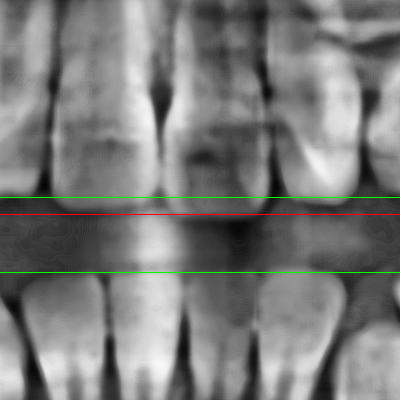
\includegraphics[width=\linewidth]{init/sep.png}
		\subcaption{Jaw separation}
	\end{minipage}
	\begin{minipage}[b]{0.32\linewidth}
		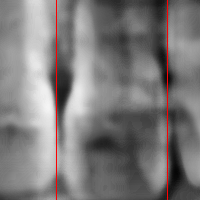
\includegraphics[width=\linewidth]{init/up.png}
		\subcaption{Upper hough lines}
	\end{minipage}
	\begin{minipage}[b]{0.32\linewidth}
		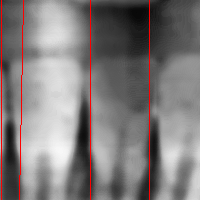
\includegraphics[width=\linewidth]{init/down.png}
		\subcaption{Lower hough lines}
	\end{minipage}
	\begin{minipage}[b]{0.32\linewidth}
		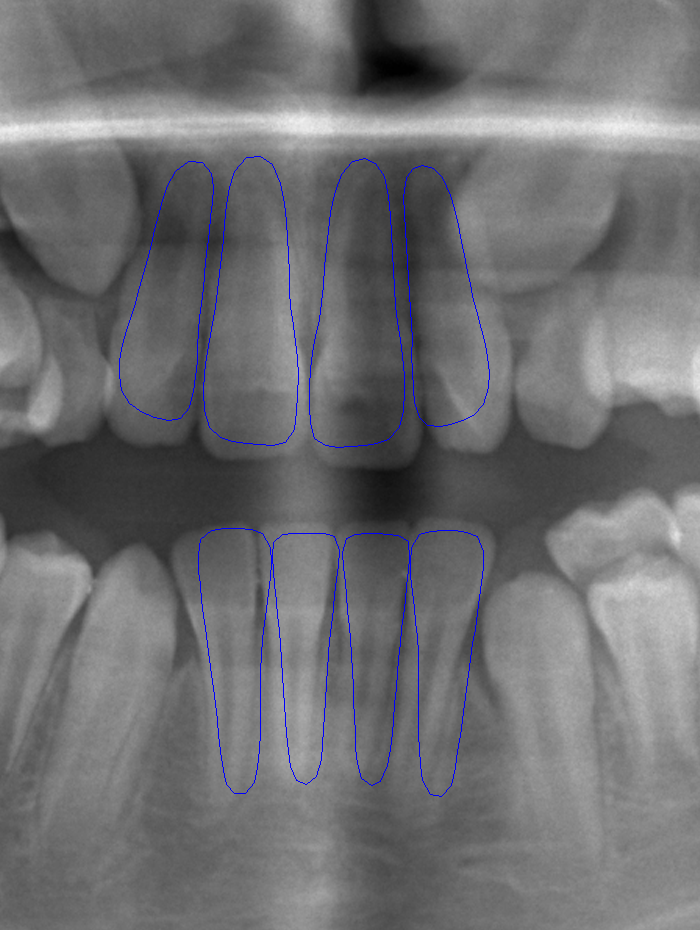
\includegraphics[width=\linewidth]{init/initial.png}
		\subcaption{Result for image 11}
	\end{minipage}
	\begin{minipage}[b]{0.32\linewidth}
		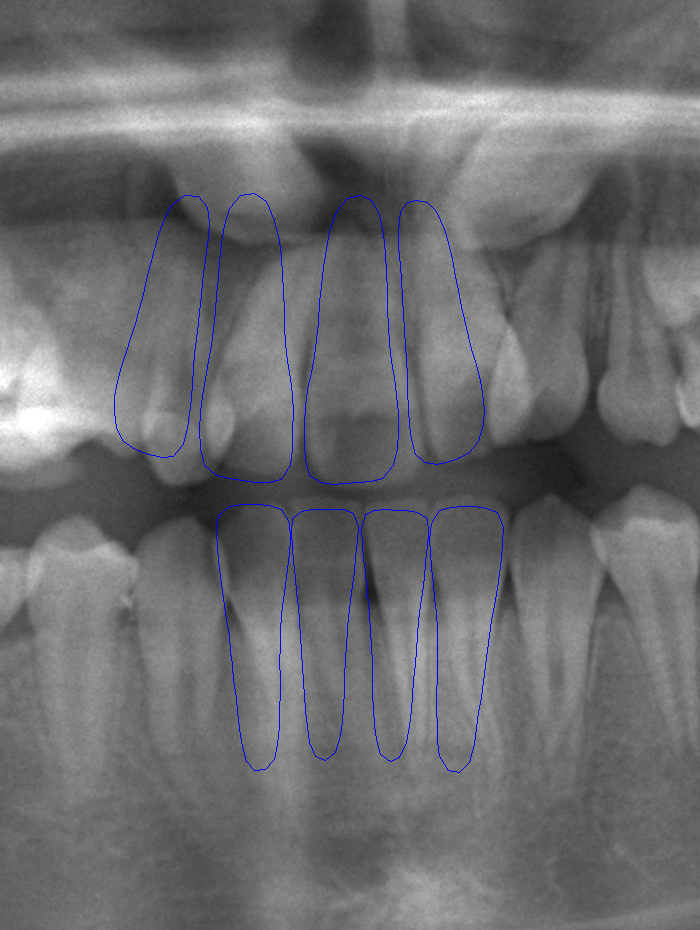
\includegraphics[width=\linewidth]{init/initial6.png}
		\subcaption{Result for image 5}
	\end{minipage}
  \caption{
		The process of getting the initial pose estimate. (a) shows the jaw separation lines for radiograph 11, where the red line shows the row of pixels with the lowest intensity and the green lines show the resulting upper and lower jaw separations.
		(b) and (c) show the hough lines for the upper and lower incisors respectively for radiograph 11.
		(d) shows the resulting initial estimate for radiograph 11, which is a really good fit, and (e) shows the initial estimate for radiograph 5.
		The estimate for radiograph 5 is a lot worse due to the off-centered position of the upper incisors.} \label{init}
\end{figure}

\subsection{The ASM algorithm}
\label{subsec:ASM}

The Active Shape Model algorithm we use to fit the model to an image closely follows the algorithm as it is described in Cootes et al \cite{cootes2000introduction}. The algorithm is reproduced here in Algorithm \ref{algo:asm}.

\begin{algorithm}
%\DontPrintSemicolon % Some LaTeX compilers require you to use \dontprintsemicolon    instead
Examine a region of the image around each point {$\textbf{X}_i$} to find the best nearby match for the point $\textbf{X}'_i$\\
Update the parameters $(X_t,Y_t,s,\theta,\textbf{b})$ to best fit the new found points \textbf{X} \\
Apply constraints to the parameters, \textbf{b}, to ensure plausible shapes (limit so $| b_i | < 3 \sqrt{\lambda_i}$)  \\
Repeat until convergence
\caption{Active Shape Model Algorithm}
\label{algo:asm}
\end{algorithm}

For the first step of the algorithm, we use a grey level model as proposed by Cootes et al \cite{cootes2000introduction}.
This is achieved by sampling $k$ pixels along the normal of a landmark on both sides, resulting in a slice with the size of $2k + 1$. This is repeated for every landmark point on every training image, after which it is combined into a statistical model for each landmark point.
The result is a mean sample and a covariance matrix for each landmark.
When looking for a new landmark point, $m > k$ pixels are sampled along the normal of a landmark point of the current estimate.
The Mahalanobis distance between the profile is then calculated to find the best nearby match.
In our implementation, some of our covariance matrices of the grey level models happened to be singular, causing the Mahalanobis distance to fail.
To alleviate this issue, we used the Moore–Penrose pseudoinverse instead of the normal inverse.
For the covariance matrices that were not singular, using the inverse or the pseudoinverse resulted in the same best nearby match, thus suggesting that these can be interchanged for our application.

For the second step of the algorithm, we used Protocol 1 as it is described by Cootes et al \cite{cootes2000introduction}.

These two steps are visualised in Figure \ref{asm}.

\begin{figure}
  \centering
	\begin{minipage}[b]{0.48\linewidth}
		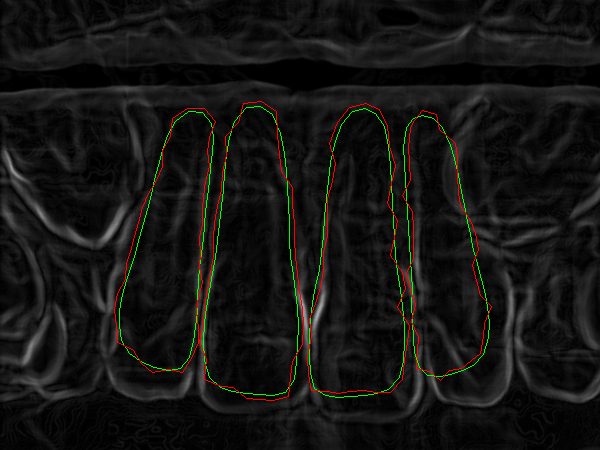
\includegraphics[width=\linewidth]{asm/step1.png}
		\subcaption{Step 1}
	\end{minipage}
	\begin{minipage}[b]{0.48\linewidth}
		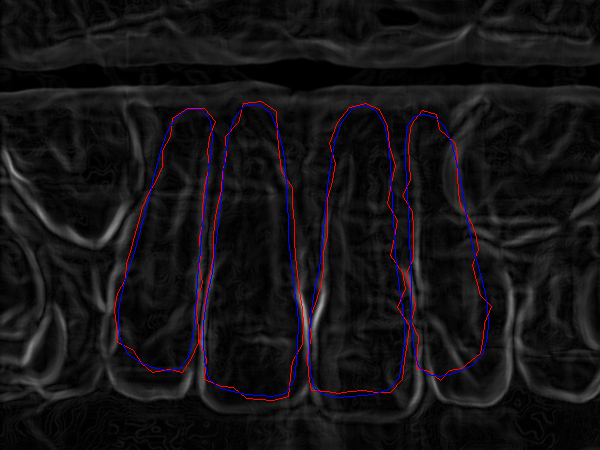
\includegraphics[width=\linewidth]{asm/step2.png}
		\subcaption{Step 2}
	\end{minipage}
  \caption{
		The two steps of the ASM algorithm for the first iteration of radiograph 11.
		(a) shows the first step, where the green shape shows the initial estimate and the red shape shows the proposed new points.
		(b) shows the second step, where the model is fitted to the red points, resulting in the blue shape.} \label{asm}
\end{figure}


\paragraph{Multi-resolution framework}
We implemented our ASM algorithm in a multi-resolution framework to improve the performance of our algorithm.
We constructed a two level Gaussian image pyramid, since returns diminished when going beyond two levels.
This allows the algorithm to first find an estimate in a coarser low resolution image, after which it is able to further fine-tune the result in the higher resolution image.

\paragraph{Stopping condition}

To determine if the ASM algorithm has converged at the current resolution, we check whether $>90\%$ of the newly proposed landmark points fall in the central $50\%$ of the $2m + 1$ slice among the previous landmark position.
We only check this for the crowns of the teeth however, as it is a lot harder for the roots to converge due to the absence of clearly defined edges.
We also allow for a maximum of 10 iterations per resolution level, as the algorithm might end up diverging when ran for a large amount of iterations.

\section{Evaluation}
\label{sec:eval}
We evaluate the performance of our algorithm using leave-one-out testing on all 14 training images. The results are marked {\color{green} green} where the solution surface overlaps with the ground truth, {\color{red} red} where the solution surface incorrectly marks an area and {\color{yellow} yellow} where the ground truth hasn't been found. 

To judge our performance, we use three measures. The Euclidian distance shows trends in performance that are correlated with properties or parameters. The miss rate indicates the percentage of ground truth we have found (and missed) and shows us that certain types of radiographs are very hard to mark. Finally, the percentage of our solution that marks the ground truth teaches us that visibility of edges is crucial. 

\subsection{Euclidian distance}
The euclidian distance between a solution and its ground truth is the total absolute distance between all corresponding landmark points. When looking for trends in the results from our experiments with varying parameter settings, we notice two main properties. The first is that increasing the number of maximum iterations our fitting procedure can take has negative effects. The boxplots in Figure \ref{fig:euclit} (a) clearly show this correlation. One example is shown in (b), where the extra allowed iterations slightly improve the lower fit but send the upper fit flying off vertically. 

Note that because of our stop condition a raised maximum number of iterations doesn't automatically mean more iterations done. Figure \ref{fig:euclit} (c) shows how many iterations were passed in each step. {\color{blue} Blue} is the subsampled upper fit, {\color{orange} orange} the full resolution upper fit, {\color{green} green} and {\color{red} red} analoguous for the lower fit. The upper model clearly runs into \texttt{maxiter} more often, implying it is fitting poorly. 

\begin{figure}
	\centering
	\begin{subfigure}{0.4\linewidth}
		\centering
		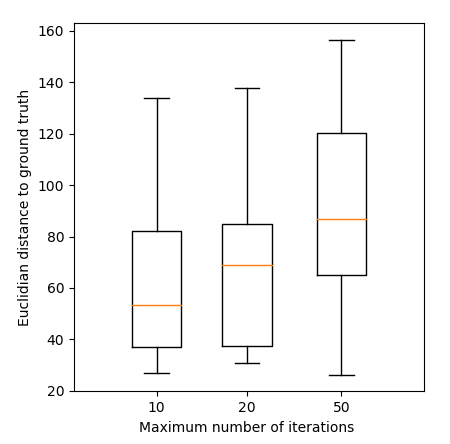
\includegraphics[width=\columnwidth]{results/chart_euclit}
		\caption{}
	\end{subfigure}
	\begin{subfigure}{0.57\linewidth}
		\centering
		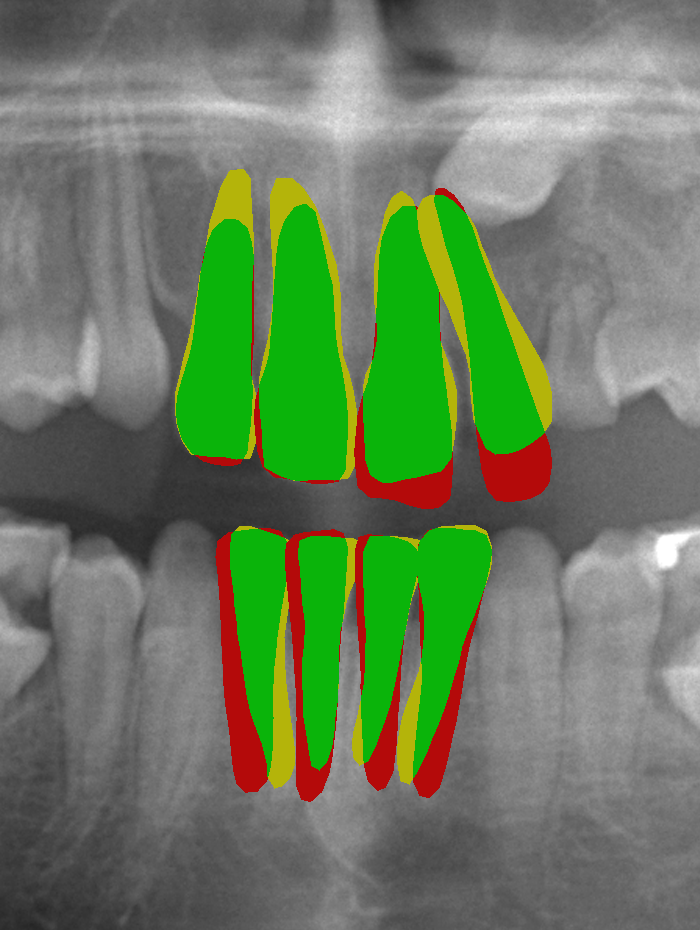
\includegraphics[width=0.45\columnwidth]{results/7i10}
		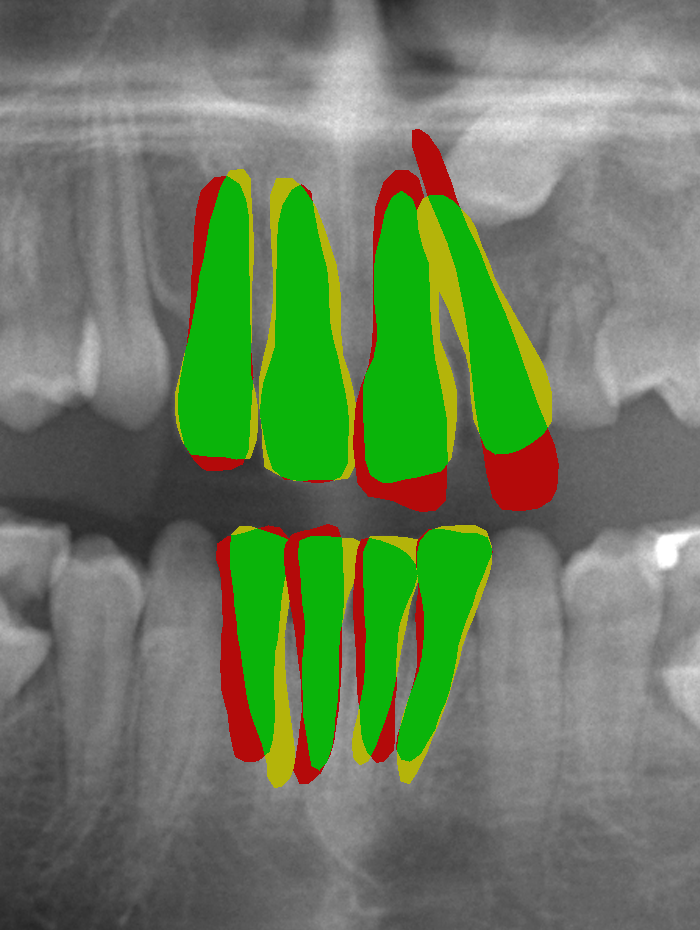
\includegraphics[width=0.45\columnwidth]{results/7i50}
		\caption{\texttt{maxiter} 10 and 50 for image 7}
	\end{subfigure}

	\begin{subfigure}{\linewidth}
		\centering
		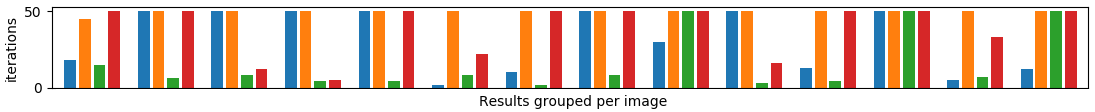
\includegraphics[width=0.98\columnwidth]{results/chart_numit}
		\caption{}
	\end{subfigure}
	\caption{Euclidian distance to the ground truth per maximum number of iterations. Longer iteration has a negative effect on performance. } %TODO plot number of it vs number max it
	\label{fig:euclit}
\end{figure}

Inspecting the boxplots in Figure \ref{fig:euclud} (a) confirms that the lower teeth are fitted generally better. This is due to a more homogeneous appearance of bottom incisors. Two examples can be found in \ref{fig:euclud} (b). Although the upper incisors have very different shapes, the lower are very similar and are marked much better as a result. 

\begin{figure}
	\centering
	\begin{subfigure}{0.32\linewidth}
		\centering
		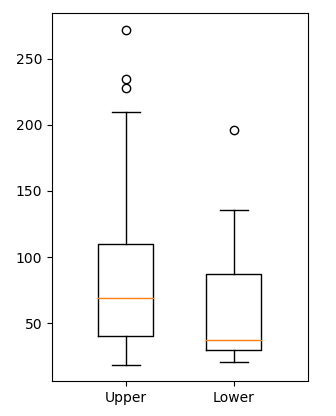
\includegraphics[width=\columnwidth]{results/chart_euclud}
		\caption{}
	\end{subfigure}
	\begin{subfigure}{0.65\linewidth}
		\centering
		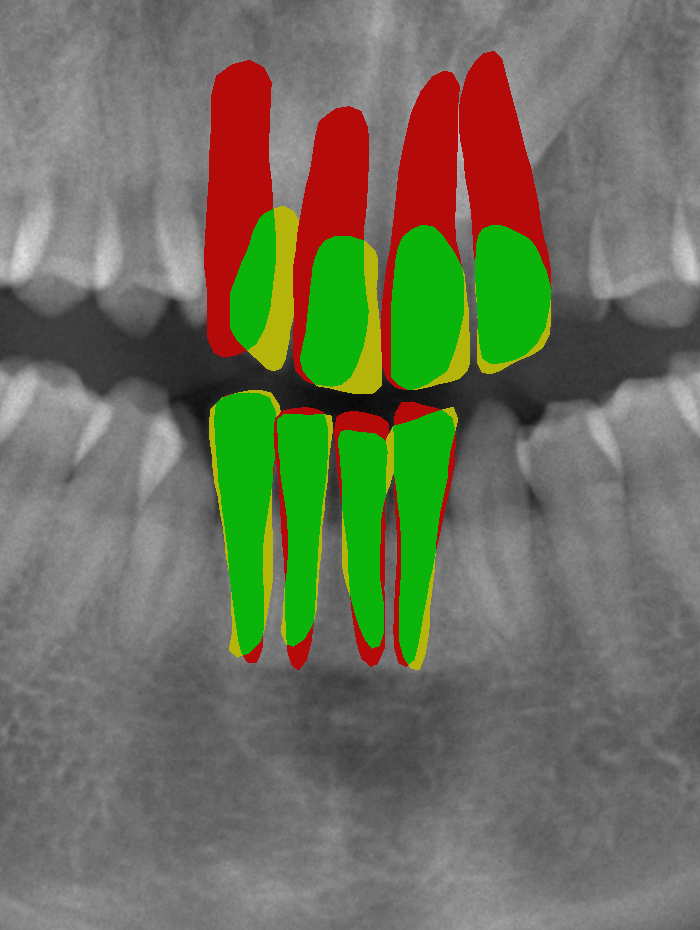
\includegraphics[width=0.45\columnwidth]{results/8i10}
		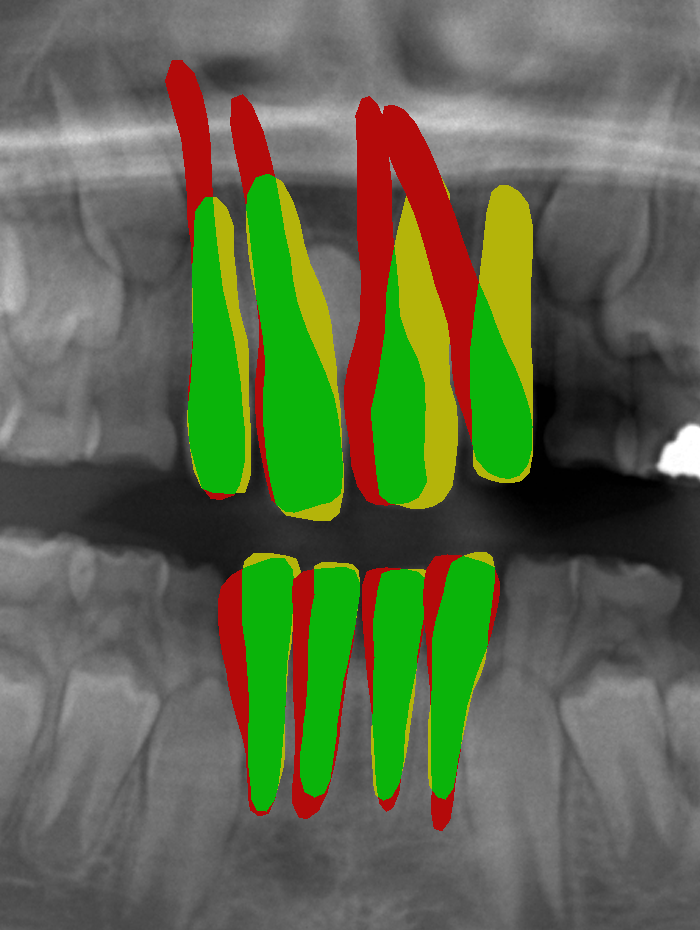
\includegraphics[width=0.45\columnwidth]{results/4i50}
		\caption{Image 8 (left) and 4 (right)}
	\end{subfigure}
	\caption{Euclidian distance to the ground truth for upper and lower models. Lower incisors appear to be more homogeneous and easier to mark. } 
	\label{fig:euclud}
\end{figure}

\subsection{Ground truth surface found}
The bar chart in Figure \ref{fig:miss} (a) shows the percentage of ground truth we have missed in our solutions. The {\color{blue} blue} bars are for the runs with 10 maximum iterations, {\color{orange} orange} for 20 iterations and {\color{green} green} for 50. We have an average miss rate of about 22\%. Some results stand out because of their high miss rate. There are two reasons for this. The first is the presence of highly visible edges due to orthodontic materials. This confuses the algorithm and pushes the iterated approximations away, as shown in subfigure (b). The second is that some radiographs are off-center by more than half a tooth, causing our initialisation to start a whole tooth to the left or right. This is shown in subfigure (c). 

\begin{figure}
	\centering
	\begin{subfigure}{\linewidth}
		\centering
		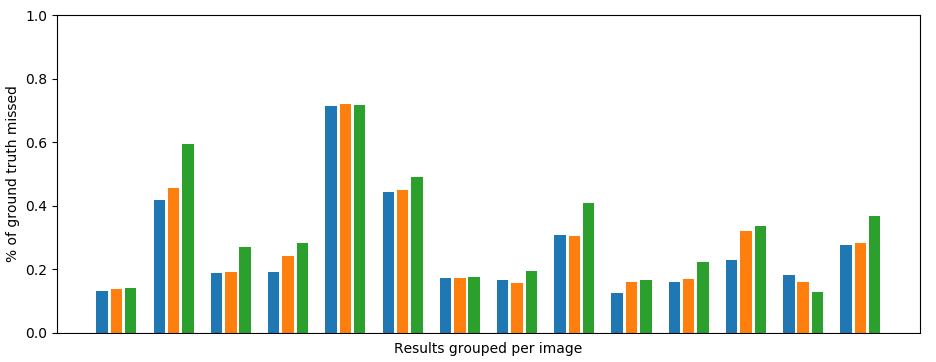
\includegraphics[width=0.8\columnwidth]{results/chart_surf2}
		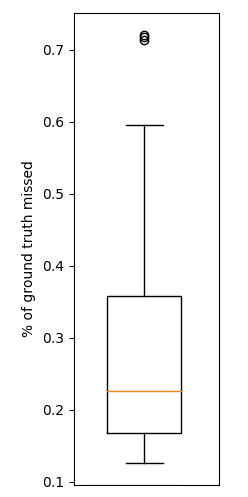
\includegraphics[width=0.15\columnwidth]{results/chart_missbox}
		\caption{}
	\end{subfigure}

	\begin{subfigure}{0.48\linewidth}
		\centering
		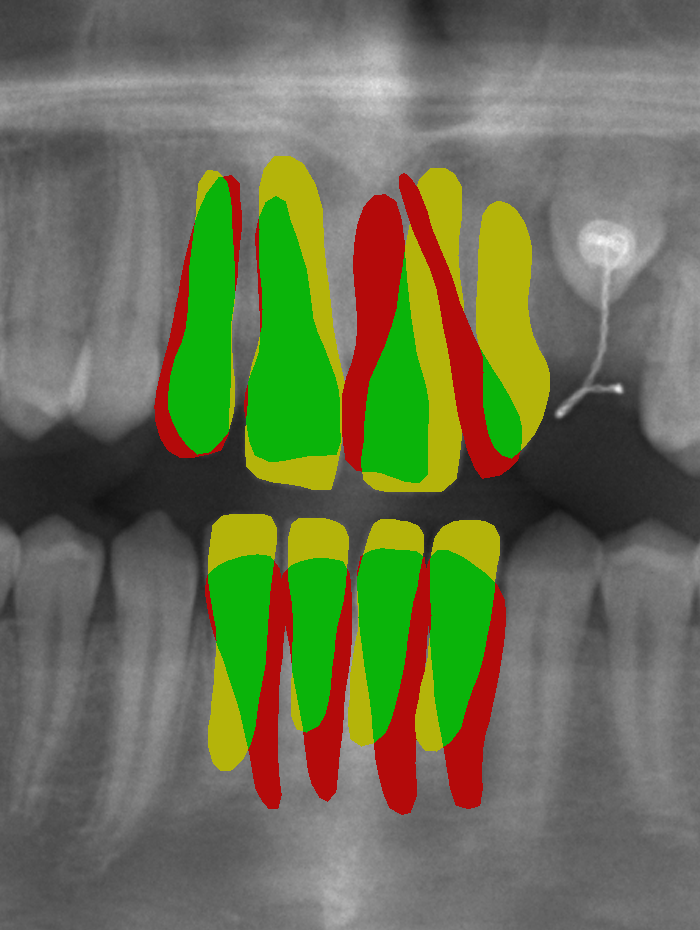
\includegraphics[width=0.48\columnwidth]{results/2i10}
		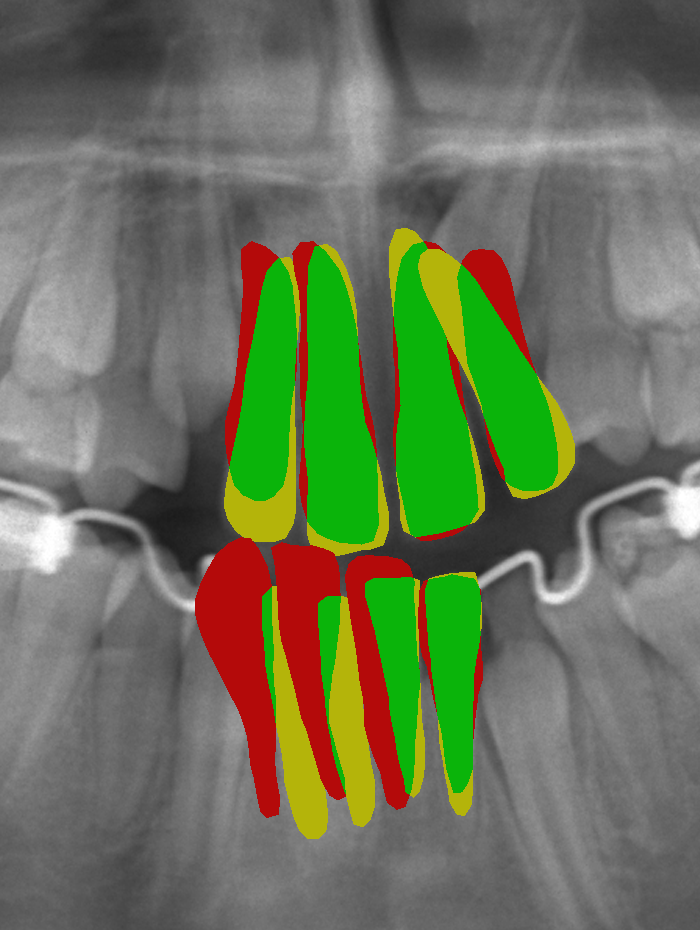
\includegraphics[width=0.48\columnwidth]{results/9i10}
		\caption{Results for images 2 and 9}
	\end{subfigure}
	\begin{subfigure}{0.48\linewidth}
		\centering
		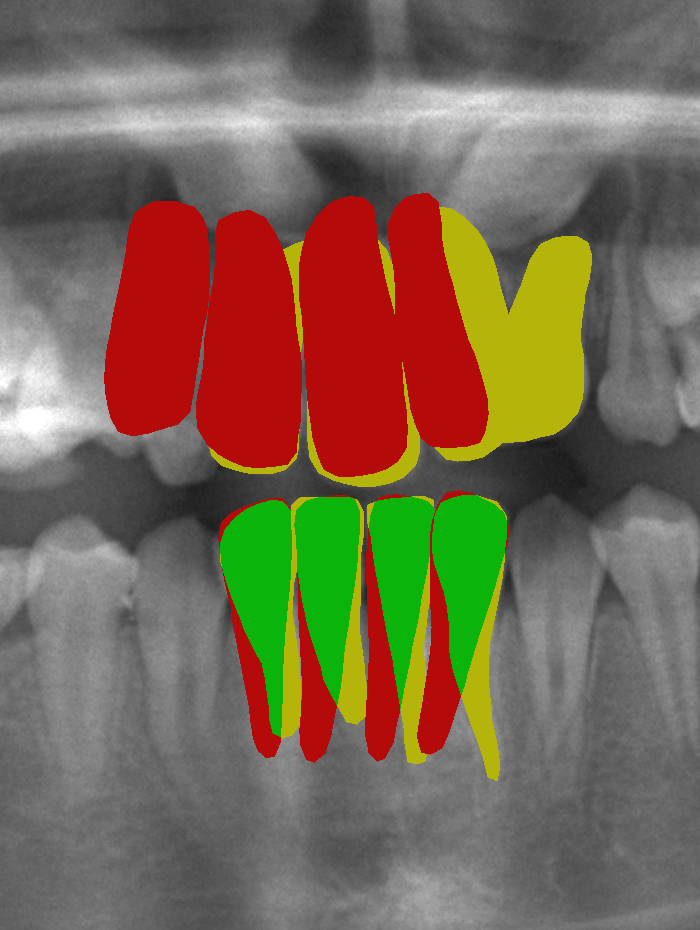
\includegraphics[width=0.48\columnwidth]{results/5i10}
		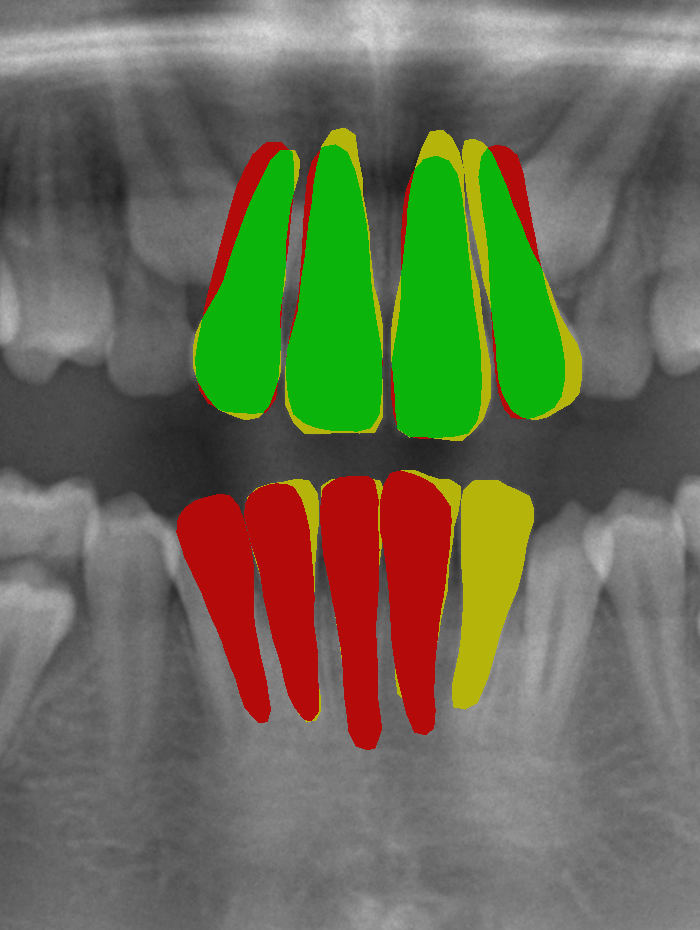
\includegraphics[width=0.48\columnwidth]{results/6i10}
		\caption{Results for images 5 and 6}
	\end{subfigure}
	\caption{Ground truth surface missed per image. Orthodontic materials and off-center initialisation causes great errors. }
	\label{fig:miss}
\end{figure}

\subsection{Correctness of solution surface}
In Figure \ref{fig:sol} (a) we show the percentage of the solution that overlaps with the ground truth. The effects of Figure \ref{fig:miss} (b) and (c) also influence this measure. However, new peaks in error rate emerge in images 8 and 12. These come from very noisy radiographs that appear almost blurred. Detecting the roots is nearly impossible. We see the result of edge detection on the enhanced images in subfigure (c) and even the manual landmark indicates only the crowns in image 8. These effects accumulate to an overall error rate of about 35\%. 

\begin{figure}
	\centering
	\begin{subfigure}{\linewidth}
		\centering
		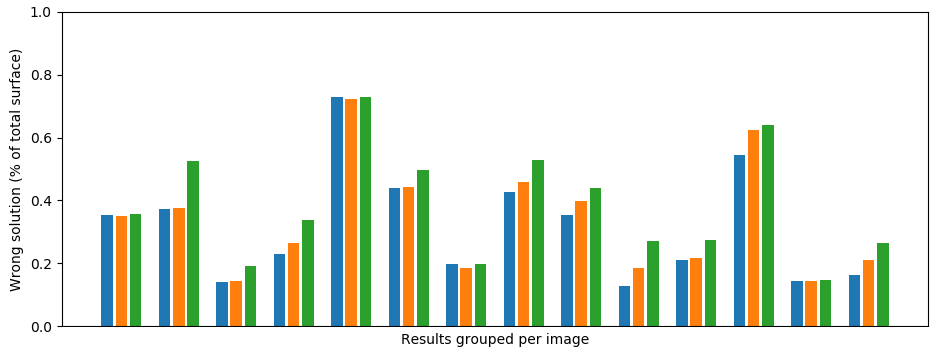
\includegraphics[width=0.8\columnwidth]{results/chart_surf4}
		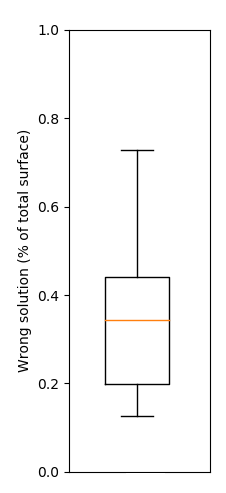
\includegraphics[width=0.15\columnwidth]{results/chart_wrongbox}
		\caption{}
	\end{subfigure}
	
	\begin{subfigure}{0.48\linewidth}
		\centering
		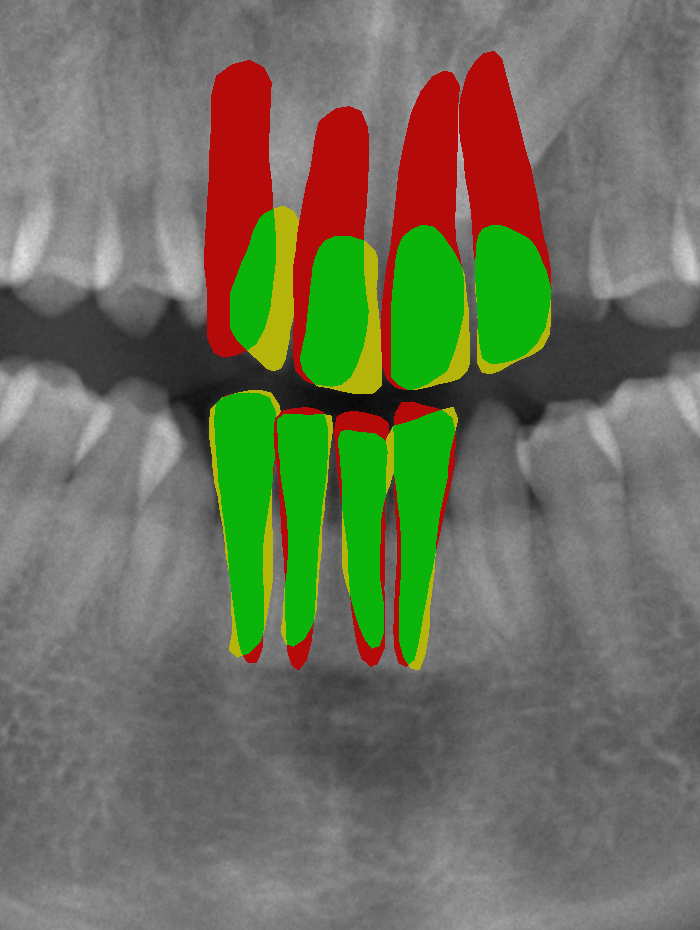
\includegraphics[width=0.48\columnwidth]{results/8i10}
		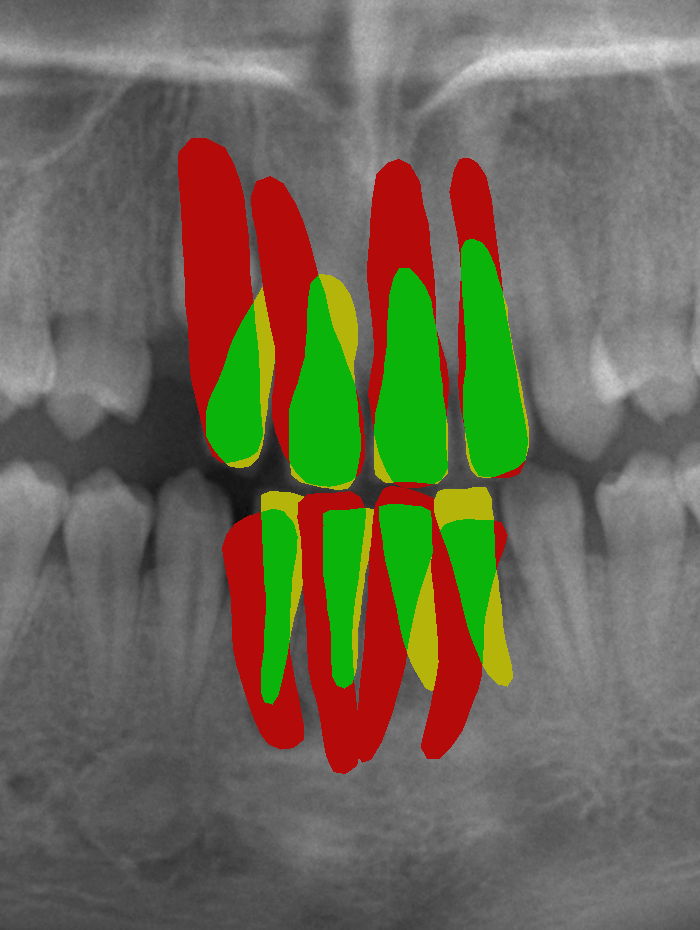
\includegraphics[width=0.48\columnwidth]{results/12i10}
		\caption{Results for images 8 and 12}
	\end{subfigure}
	\begin{subfigure}{0.48\linewidth}
		\centering
		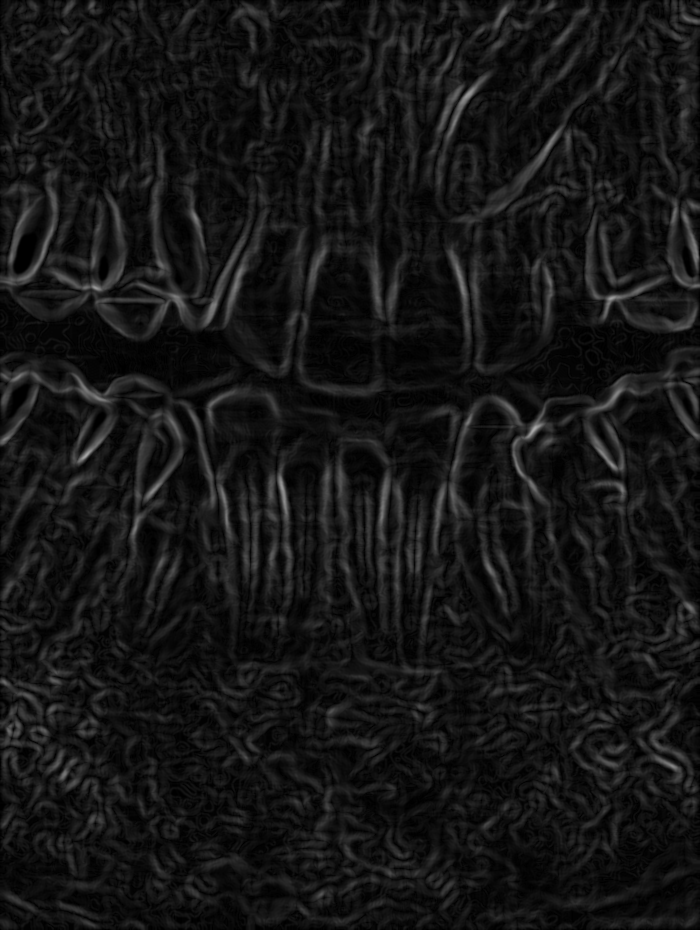
\includegraphics[width=0.48\columnwidth]{results/8sobel}
		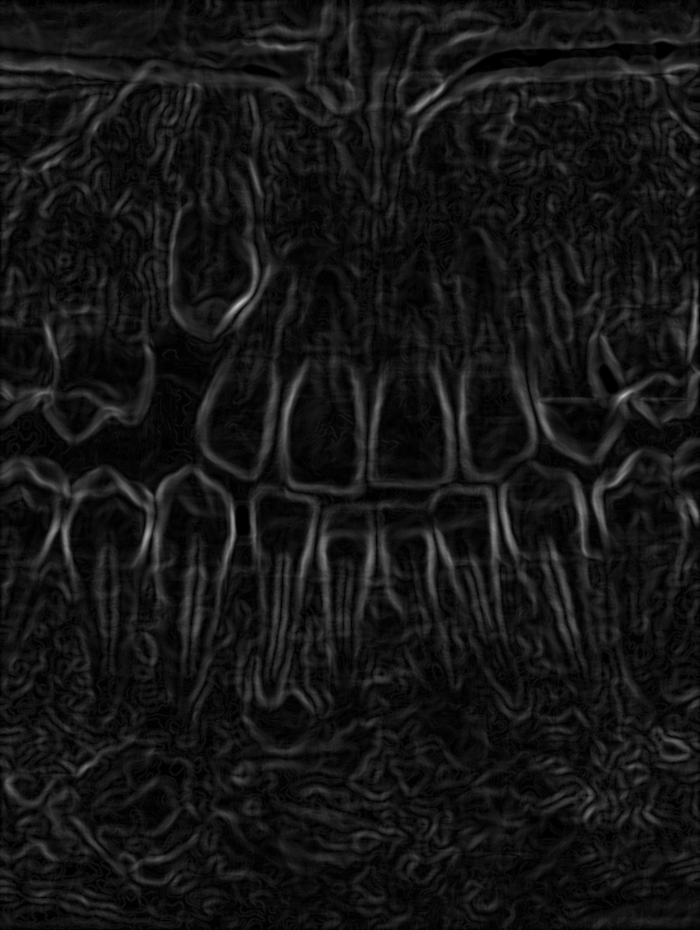
\includegraphics[width=0.48\columnwidth]{results/12sobel}
		\caption{Sobel edges for images 8 and 12}
	\end{subfigure}
	\caption{Erroneous solution surface per image. Poorly visible incisor roots cause the approximation to fly off. }
	\label{fig:sol}
\end{figure}

\bibliography{references}
\bibliographystyle{plain}

\end{document}
